The results of the background estimation and associated uncertainties
are summarized in
Table~\ref{tab:results_zerojet},~\ref{tab:results_1jet}
and~\ref{tab:results_vbf}.

We compute the upper limits with a Bayesian method assuming a flat
prior~\ref{blah} using the software package LandS.

The upper limit are shown in Figure~\ref{fig:cutbase_zerojet} and
summarized Table~\ref{tab:blah}.

\begin{table}[!ht]
  \begin{center}
 {\footnotesize
  \begin{tabular} {|c|c|c|c|c|c|c|c|}
  \hline
  & DY+X (data) & top & Wjets & WW & Other Bkg MC & H$_{120}$ & Data \\
  \hline
  mm & $xx \pm yy \pm zz$ & $xx \pm yy \pm zz$ & $xx \pm yy \pm zz$ & $xx \pm yy \pm zz$ & $xx \pm yy \pm zz$ & $xx \pm yy \pm zz$ & $xx \pm yy \pm zz$ \\
  me & $xx \pm yy \pm zz$ & $xx \pm yy \pm zz$ & $xx \pm yy \pm zz$ & $xx \pm yy \pm zz$ & $xx \pm yy \pm zz$ & $xx \pm yy \pm zz$ & $xx \pm yy \pm zz$ \\
  em & $xx \pm yy \pm zz$ & $xx \pm yy \pm zz$ & $xx \pm yy \pm zz$ & $xx \pm yy \pm zz$ & $xx \pm yy \pm zz$ & $xx \pm yy \pm zz$ & $xx \pm yy \pm zz$ \\
  ee & $xx \pm yy \pm zz$ & $xx \pm yy \pm zz$ & $xx \pm yy \pm zz$ & $xx \pm yy \pm zz$ & $xx \pm yy \pm zz$ & $xx \pm yy \pm zz$ & $xx \pm yy \pm zz$ \\
  \hline
  \hline
  & DY+X (data) & top & Wjets & WW & Other Bkg MC & H$_{130}$ & Data \\
  \hline
  mm & $xx \pm yy \pm zz$ & $xx \pm yy \pm zz$ & $xx \pm yy \pm zz$ & $xx \pm yy \pm zz$ & $xx \pm yy \pm zz$ & $xx \pm yy \pm zz$ & $xx \pm yy \pm zz$ \\
  me & $xx \pm yy \pm zz$ & $xx \pm yy \pm zz$ & $xx \pm yy \pm zz$ & $xx \pm yy \pm zz$ & $xx \pm yy \pm zz$ & $xx \pm yy \pm zz$ & $xx \pm yy \pm zz$ \\
  em & $xx \pm yy \pm zz$ & $xx \pm yy \pm zz$ & $xx \pm yy \pm zz$ & $xx \pm yy \pm zz$ & $xx \pm yy \pm zz$ & $xx \pm yy \pm zz$ & $xx \pm yy \pm zz$ \\
  ee & $xx \pm yy \pm zz$ & $xx \pm yy \pm zz$ & $xx \pm yy \pm zz$ & $xx \pm yy \pm zz$ & $xx \pm yy \pm zz$ & $xx \pm yy \pm zz$ & $xx \pm yy \pm zz$ \\
  \hline
  \end{tabular}
  }
  \caption{Expected number of signal and background events for an 
  integrated luminosity of 1\ifb{} after 
  applying the \ww\ 0-jet selection requirements. Monte Carlo statistical uncertainties are 
  included.}
   \label{tab:results_zerojet}
  \end{center}
\end{table}

\begin{figure}[!htbp]
\begin{center}
   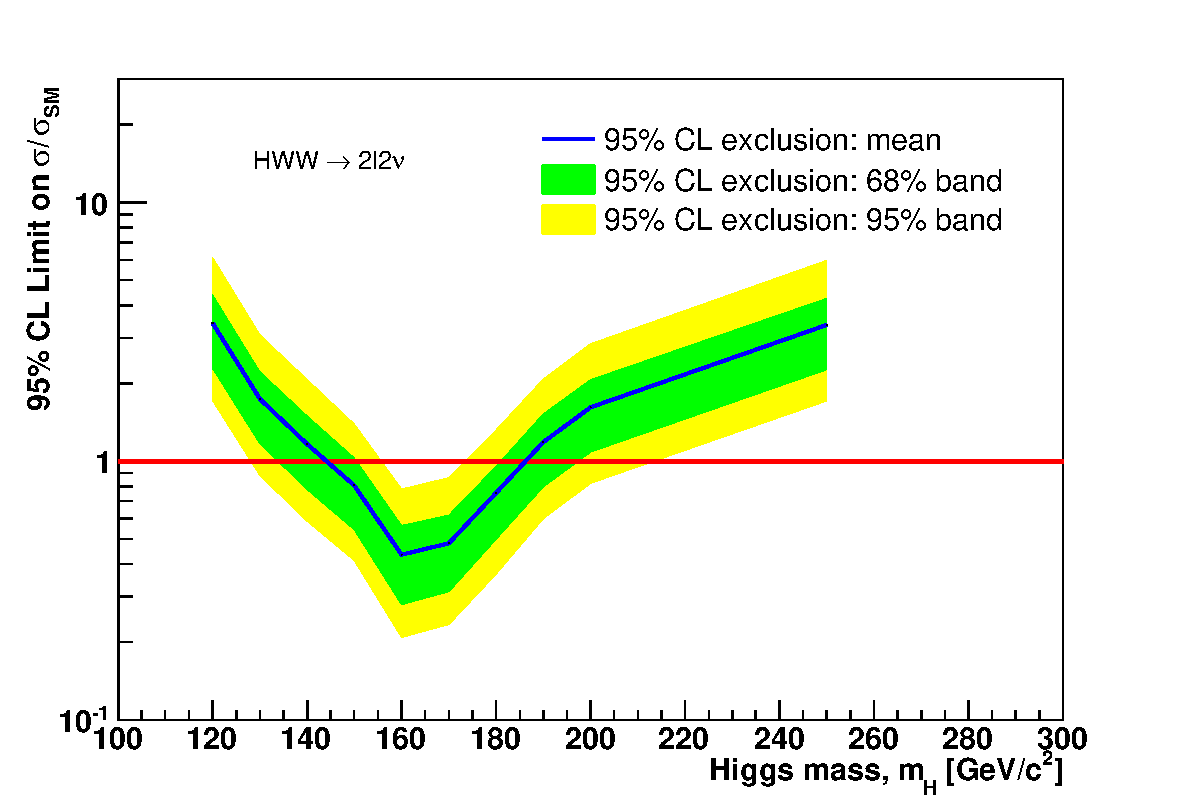
\includegraphics[width=0.9\textwidth]{figures/cut_based_limits.pdf}
   \caption{Cut based analysis expected upper limits at 95\%C.L. for 1\ifb\ of data.}
   \label{fig:cutbase_uls}
\end{center}
\end{figure}
